\chapter{Les organomagnésiens}\label{ch:b1:organomagnesium}

La plupart des molécules organiques utiles comptent plus d'atomes de
carbone que n'importe quelle matière première bon marché, et le problème
central de la synthèse est de relier deux squelettes carbonés par une
nouvelle liaison C--C. Dans un composé carboné, le carbone est presque
toujours le partenaire pauvre en électrons d'une liaison --- avec
l'oxygène, avec un halogène --- et deux carbones pauvres en électrons ne
réagissent pas entre eux. Au tournant du vingtième siècle, un réactif
préparé dans un seul ballon à partir d'un halogénoalcane et de magnésium
a renversé la situation~: son carbone est riche en électrons, c'est un
\omterm{def:b1:electronic-effects:nucleophile}{nucléophile} qui attaque le carbone d'un groupe carbonyle. Grâce à lui,
on peut construire des alcools de presque tous les squelettes à partir
de fragments plus petits. Ce chapitre montre comment on prépare ce
réactif, pourquoi il exige un ballon parfaitement sec, sur quoi il
s'additionne, et comment s'en servir pour planifier une synthèse.

\begin{recall}
L'\omterm{def:b1:periodicity:electronegativity}{électronégativité} (\cref{ch:b1:periodicity})~; les acides et les \omterm{def:b1:lewis-resonance-vsepr:lewis-acid}{bases
de Lewis} et la \omterm{def:b1:lewis-resonance-vsepr:lewis-acid}{liaison dative} (\cref{ch:b1:lewis-resonance-vsepr})~; les
\omterm{def:b1:electronic-effects:nucleophile}{nucléophiles}, les \omterm{def:b1:electronic-effects:nucleophile}{électrophiles}, les \omterm{def:b1:electronic-effects:curly-arrow}{flèches courbes} et l'échelle des
$\mathrm{p}K_a$ des espèces organiques (\cref{ch:b1:electronic-effects})~;
la classe d'un alcool (primaire, secondaire, tertiaire) est celle de son
carbone.
\end{recall}

\section{Préparer un réactif de Grignard}

\begin{definition}[Composé organométallique, réactif de Grignard]\label{def:b1:organomagnesium:organometallic}
Un \emph{composé organométallique}\index{compose organometallique@composé organométallique} comporte au moins
une liaison carbone--métal. Un \emph{organomagnésien}\index{organomagnesien@organomagnésien}
possède une liaison C--Mg~; le \emph{réactif de
Grignard}\index{reactif de Grignard@réactif de Grignard} \ce{RMgX} (X = Cl, Br, I), préparé à partir d'un
halogénoalcane ou d'un halogénoarène et de magnésium dans un éther,
\ce{R-X + Mg -> R-MgX}, est le plus courant.
\end{definition}

Le magnésium s'insère dans la liaison C--X. L'éther n'est pas un solvant
innocent~: dans \ce{RMgX}, le magnésium n'est entouré que de quatre
\omterm{def:b1:quantum-numbers:configuration}{électrons de valence}, et deux molécules d'éther lui cèdent leurs
\omterm{def:b1:lewis-resonance-vsepr:lewis}{doublets non liants}, ce qui complète son octet et maintient le réactif en
solution.

\begin{omfigure}
\begin{tikzpicture}[font=\small]
  \node (mg) at (0,0) {Mg};
  \node (r) at (-1.5,0) {R};
  \node (x) at (1.5,0) {Br};
  \node (o1) at (0,1.45) {O};
  \node (o2) at (0,-1.45) {O};
  \draw[thick] (r) -- (mg) -- (x);
  \draw[thick, ->, omDef] (o1) -- (mg);
  \draw[thick, ->, omDef] (o2) -- (mg);
  \draw (o1) -- ++(-0.8,0.45) node[left] {\ce{CH3CH2}};
  \draw (o1) -- ++(0.8,0.45) node[right] {\ce{CH2CH3}};
  \draw (o2) -- ++(-0.8,-0.45) node[left] {\ce{CH3CH2}};
  \draw (o2) -- ++(0.8,-0.45) node[right] {\ce{CH2CH3}};
  \node[align=left, anchor=west] at (3.2,0) {deux molécules d'éther cèdent\\chacune un doublet (en bleu)~:\\magnésium tétraédrique,\\un octet d'électrons};
\end{tikzpicture}

{\small Un \omterm{def:b1:organomagnesium:organometallic}{réactif de Grignard} dans l'éthoxyéthane (éther diéthylique).
Les \omterm{def:b1:lewis-resonance-vsepr:lewis-acid}{liaisons datives} oxygène--magnésium expliquent pourquoi le réactif ne
se forme que dans un éther ou dans une \omterm{def:b1:lewis-resonance-vsepr:lewis-acid}{base de Lewis} analogue.}
\end{omfigure}

\begin{method}[Préparer un réactif de Grignard]\label{met:b1:organomagnesium:prepare}
\begin{enumerate}
  \item Sécher toute la verrerie à l'étuve~; munir le réfrigérant d'une
        garde à chlorure de calcium~; utiliser un éther anhydre.
  \item Placer les tournures de magnésium et un peu d'éther dans un
        ballon tricol muni d'un réfrigérant, d'une ampoule de coulée et
        d'un agitateur.
  \item Ajouter une petite portion de l'halogénure~; lorsque la réaction
        démarre (trouble, ébullition douce de l'éther), ajouter le reste
        goutte à goutte, à un rythme qui maintient un léger reflux.
  \item Utiliser la solution aussitôt, dans le même montage sec.
\end{enumerate}
\end{method}

\begin{omfigure}
\begin{tikzpicture}[font=\small]
  \pic at (0,-0.05) {stirrer};
  \pic (f) at (0,0.05) {threeneck={0.35}{omDef!14}};
  \pic at (f-c) {condenser};
  \pic at ($(f-c)+(0,3.2)$) {guardtube};
  \pic[rotate=25] at (f-l) {dropfunnel={0.5}{orange!20}};
  \fill[black!45, rotate around={-25:(f-r)}] ($(f-r)+(-0.17,0)$) rectangle ++(0.34,0.3);
  \draw[->] (2.4,0.9) node[right] {tournures de Mg dans l'éther anhydre} -- (0.6,0.6);
  \draw[->] (-3.0,3.9) node[left, align=right] {halogénure dans l'éther,\\ajouté goutte à goutte} -- (-1.8,3.4);
  \draw[->] (1.8,5.3) node[right] {réfrigérant (eau)} -- (0.45,4.8);
  \draw[->] (1.8,6.6) node[right] {garde à chlorure de calcium} -- (0.3,6.4);
  \draw[->] (2.4,-0.2) node[right] {agitateur magnétique} -- (1.3,-0.2);
\end{tikzpicture}

{\small Montage pour une réaction de Grignard~: tout ce que l'air peut
atteindre est séché. La vapeur d'eau de l'air est arrêtée par la garde~;
le réfrigérant renvoie dans le ballon l'éther en ébullition.}
\end{omfigure}

\begin{inthelab}[Une réaction qui doit démarrer]
Une préparation de Grignard refuse parfois de démarrer~: le magnésium est
recouvert d'une couche d'oxyde. Écraser une tournure avec un agitateur
en verre, ajouter un \omterm{def:b1:crystals-metals:crystal}{cristal} de diiode ou chauffer localement le ballon
met à nu du métal frais. Une fois lancée, la réaction est exothermique et
l'éther bout de lui-même~; on ralentit alors l'ajout pour éviter le
débordement. L'éthoxyéthane bout à \qty{35}{\celsius} et sa vapeur est
très inflammable~: aucune flamme dans le laboratoire, et un bain de glace
à portée de main.
% ledger: bp:diethylether
\end{inthelab}

\section{Une base forte et un nucléophile}

\begin{definition}[Inversion de polarité]\label{def:b1:organomagnesium:umpolung}
L'\omterm{def:b1:periodicity:electronegativity}{électronégativité} du magnésium (1.31) est bien plus faible que celle
du carbone (2.55)~: dans \ce{R-MgX}, la liaison C--Mg est polarisée avec
l'extrémité négative sur le carbone, qui se comporte comme un
\omterm{def:b1:electronic-effects:intermediates}{carbanion}. Dans l'halogénure \ce{R-X}, le même carbone était positif
(X~: 2.96 pour Br). Transformer un carbone \omterm{def:b1:electronic-effects:nucleophile}{électrophile} en carbone
\omterm{def:b1:electronic-effects:nucleophile}{nucléophile} est une \emph{inversion de polarité}\index{inversion de polarite@inversion de polarité}.
% ledger: en:Mg, en:C, en:Br
\end{definition}

\begin{proposition}[Les réactifs de Grignard sont détruits par les hydrogènes acides]\label{prop:b1:organomagnesium:base}
Un \omterm{def:b1:organomagnesium:organometallic}{réactif de Grignard} réagit quantitativement avec l'eau, les alcools,
les acides carboxyliques, les amines porteuses de liaisons N--H et les
alcynes terminaux, en donnant l'alcane
\ce{R-H}~: \ce{RMgX + H2O -> R-H + Mg(OH)X}.
\end{proposition}

\begin{proof}
Le carbone de type \omterm{def:b1:electronic-effects:intermediates}{carbanion} est la base du couple \ce{R-H}/\ce{R^-}, et
les alcanes sont de loin les acides les plus faibles de la chimie
organique~: on ne peut mesurer aucun départ de proton dans l'eau, où
l'hydroxyde est la base la plus forte qui puisse exister
(\cref{ch:b1:predominant-reaction}, \omterm{def:b1:predominant-reaction:levelling}{effet nivelant}). Tous les acides de
la liste sont beaucoup plus forts, et le transfert de proton vers
\ce{R^-} a une constante énorme~: il est total et rapide.
\end{proof}

C'est la raison du montage sec~: une goutte d'eau détruit une quantité
égale de réactif. Transformé en atout, \ce{CH3CH2MgBr + D2O} place un
atome de deutérium exactement là où se trouvait le brome.

\section{Additions sur les composés carbonylés et sur le dioxyde de carbone}

Le carbone d'un groupe C=O est \omterm{def:b1:electronic-effects:nucleophile}{électrophile}
(\cref{ch:b1:electronic-effects}). Le \omterm{def:b1:organomagnesium:organometallic}{réactif de Grignard} lui ajoute son
groupe R, le doublet $\pi$ de C=O passant sur l'oxygène~; une hydrolyse
acide protone ensuite l'alcoolate.

\begin{omfigure}
\setchemfig{atom sep=2.1em}
\schemestart
\chemfig{@{r}R-[@{rm}]MgBr}
\+
\chemfig{@{cc}C(-[:150]R')(-[:210]R'')=[@{co}]@{o}O}
\arrow{->}
\chemfig{C(-[:150]R')(-[:210]R'')(-[2]R)-O^{-}}
\chemfig{\phantom{.}}\chemfig{^{+}MgBr}
\arrow{->[\ce{H3O+}]}
\chemfig{C(-[:150]R')(-[:210]R'')(-[2]R)-OH}
\schemestop
\chemmove{\draw[->, thick, shorten <=2pt, shorten >=2pt](rm) .. controls +(70:9mm) and +(180:7mm) .. (cc);
          \draw[->, thick, shorten <=2pt, shorten >=2pt](co) .. controls +(90:6mm) and +(90:6mm) .. (o);}
\par\vspace{6pt}

{\small Addition d'un \omterm{def:b1:organomagnesium:organometallic}{réactif de Grignard} sur une cétone (ou un aldéhyde,
$\mathrm{R''} = \mathrm{H}$)~: le doublet de C--Mg forme la nouvelle liaison C--C pendant que
le doublet $\pi$ de C=O passe sur l'oxygène~; l'alcoolate de magnésium
est protoné par un acide dilué dans une étape séparée.}
\end{omfigure}

\begin{proposition}[Des alcools à partir des composés carbonylés]\label{prop:b1:organomagnesium:carbonyl-addition}
Après hydrolyse acide, un \omterm{def:b1:organomagnesium:organometallic}{réactif de Grignard} \ce{RMgX} donne~: avec le
méthanal, un alcool primaire \ce{RCH2OH}~; avec un autre aldéhyde
$\mathrm{R'CHO}$, un alcool secondaire $\mathrm{RR'CHOH}$~; avec une
cétone $\mathrm{R'COR''}$, un alcool tertiaire
$\mathrm{RR'R''COH}$. La nouvelle liaison C--C relie R à l'ancien carbone
du carbonyle.
\end{proposition}

\begin{proof}
Le carbone du carbonyle conserve ses deux substituants et gagne R et un
OH (venant de l'oxygène de l'alcoolate)~: le méthanal apporte deux H, un
aldéhyde un H et un groupe carboné, une cétone deux groupes carbonés. La
classe de l'alcool est le nombre de groupes carbonés portés par ce
carbone~: un, deux ou trois.
\end{proof}

\begin{proposition}[Des acides carboxyliques à partir du dioxyde de carbone]\label{prop:b1:organomagnesium:co2}
Un \omterm{def:b1:organomagnesium:organometallic}{réactif de Grignard} versé sur du dioxyde de carbone solide donne,
après acidification, l'acide carboxylique \ce{RCOOH}, qui compte un
carbone de plus~:
\ce{RMgX + CO2 -> RCOOMgX}, puis \ce{RCOOMgX + H3O+ -> RCOOH + Mg^2+ + X- + H2O}.
\end{proposition}

\begin{proof}
\ce{CO2} est un composé carbonylé dont le carbone est attaqué comme
celui d'une cétone~; le carboxylate formé est trop peu réactif pour
additionner un second groupe R dans ces conditions (un carbonyle chargé
négativement est un mauvais \omterm{def:b1:electronic-effects:nucleophile}{électrophile}). L'acide le protone.
\end{proof}

\section{Construire des squelettes carbonés}

\begin{method}[Planifier la synthèse d'un alcool]\label{met:b1:organomagnesium:plan-alcohol}
\begin{enumerate}
  \item Repérer le carbone qui porte le OH dans l'alcool cible.
  \item Choisir l'un de ses groupes carbonés comme R (il viendra du
        \omterm{def:b1:organomagnesium:organometallic}{réactif de Grignard}, préparé à partir de \ce{R-Br})~; le reste de
        la molécule, avec ce carbone sous forme de C=O, est le partenaire
        carbonylé.
  \item Recenser les choix possibles (un par groupe carboné) et préférer
        celui qui fait appel à des réactifs simples et disponibles.
  \item Vérifier qu'aucun des partenaires ne porte d'hydrogène acide ni
        de second carbonyle qui réagirait aussi.
\end{enumerate}
\end{method}

\begin{example}[Le 2-phénylbutan-2-ol]\label{ex:b1:organomagnesium:plan}
Le carbone qui porte le OH porte un groupe phényle, un groupe méthyle et
un groupe éthyle. Trois choix~: le bromure de phénylmagnésium avec la
butan-2-one~; le bromure de méthylmagnésium avec la
1-phénylpropan-1-one~; le bromure d'éthylmagnésium avec la
1-phényléthan-1-one (acétophénone). Les trois conviennent~; le dernier
utilise deux des réactifs les plus courants.
\end{example}

\begin{history}[Victor Grignard]
\begin{minipage}[t]{0.2\linewidth}\vspace{0pt}
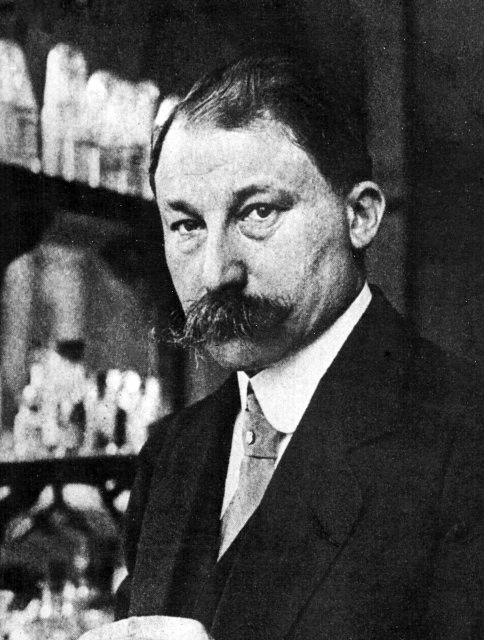
\includegraphics[width=\linewidth]{images/book2/grignard.jpg}
\end{minipage}\hfill
\begin{minipage}[t]{0.76\linewidth}\vspace{0pt}
Le réactif porte le nom de Victor Grignard, qui, doctorant au tournant
du vingtième siècle, découvrit que le magnésium se dissout dans une
solution éthérée d'halogénoalcane et que la solution s'additionne sur
les composés carbonylés. Sa simplicité --- un métal, un solvant, un
ballon --- en fit la réaction de formation de liaison carbone--carbone
la plus utilisée du siècle, et valut à son découvreur un prix Nobel de
chimie. (Photographie, domaine public, Wikimedia Commons.)
\end{minipage}
\end{history}

\section{Exercices}

\begin{exercise}[$\star$]\label{exo:b1:organomagnesium:1}
Écrire la préparation du bromure d'éthylmagnésium et du bromure de
phénylmagnésium. Donner la polarisation de la liaison C--Br et de la
liaison C--Mg, avec les \omterm{def:b1:periodicity:electronegativity}{électronégativités}.
\end{exercise}

\begin{exercise}[$\star$]\label{exo:b1:organomagnesium:2}
Que donne l'iodure de méthylmagnésium avec~: l'eau~; l'éthanol~;
l'acide éthanoïque~; l'oxyde de deutérium \ce{D2O}~? Écrire les
équations.
\end{exercise}

\begin{exercise}[$\star$]\label{exo:b1:organomagnesium:3}
Donner le produit (après hydrolyse acide) du bromure d'éthylmagnésium
avec le méthanal, l'éthanal, la propanone, le benzaldéhyde et le dioxyde
de carbone. Donner la classe de chaque alcool.
\end{exercise}

\begin{exercise}[$\star$]\label{exo:b1:organomagnesium:4}
Pourquoi ne faut-il pas utiliser le 4-bromobutan-1-ol pour préparer un
\omterm{def:b1:organomagnesium:organometallic}{réactif de Grignard}~?
\end{exercise}

\begin{exercise}[$\star\star$]\label{exo:b1:organomagnesium:5}
Écrire le mécanisme de l'addition du bromure de méthylmagnésium sur
l'éthanal et de l'hydrolyse, avec les \omterm{def:b1:electronic-effects:curly-arrow}{flèches courbes}. Le produit est-il
\omterm{def:b1:stereochemistry-in-depth:stereocentre}{chiral}~? Est-il obtenu sous forme d'un seul énantiomère~? Pourquoi~?
\end{exercise}

\begin{exercise}[$\star\star$]\label{exo:b1:organomagnesium:6}
Proposer deux façons de préparer le 3-méthylpentan-3-ol à partir d'un
\omterm{def:b1:organomagnesium:organometallic}{réactif de Grignard} et d'une cétone.
\end{exercise}

\begin{exercise}[$\star\star$]\label{exo:b1:organomagnesium:7}
Comment préparer l'acide 2-méthylpropanoïque à partir du
2-bromopropane~? Calculer la masse d'acide obtenue à partir de
\qty{12.3}{g} de bromure avec un \omterm{def:b1:extent-q-and-k:fractional-extent}{rendement} de \qty{70}{\percent}
($M$~: \ce{C3H7Br} \qty{123.0}{g/mol}, \ce{C4H8O2}
\qty{88.0}{g/mol}).
\end{exercise}

\begin{exercise}[$\star\star$]\label{exo:b1:organomagnesium:8}
Un étudiant négligent prépare du bromure de phénylmagnésium à partir de
\qty{0.0500}{mol} de bromobenzène dans un éther contenant \qty{0.18}{g}
d'eau. Quelle fraction du réactif est détruite~? Quel produit se
forme~?
\end{exercise}

\begin{exercise}[$\star\star$]\label{exo:b1:organomagnesium:9}
Le biphényle, \ce{C6H5-C6H5}, est un sous-produit de la préparation du
bromure de phénylmagnésium. Proposer un mode de formation, et expliquer
pourquoi l'ajout lent du bromobenzène sur un excès de magnésium le
limite.
\end{exercise}

\begin{exercise}[$\star\star\star$]\label{exo:b1:organomagnesium:10}
Planifier deux synthèses du 1-phényléthan-1-ol à partir d'un \omterm{def:b1:organomagnesium:organometallic}{réactif de
Grignard}, et une synthèse du 2-phénylpropan-2-ol. Pour chacune, nommer
l'halogénure qui donne le réactif.
\end{exercise}

\begin{exercise}[$\star\star\star$]\label{exo:b1:organomagnesium:11}
Expliquer pourquoi le \omterm{def:b1:organomagnesium:organometallic}{réactif de Grignard} et le composé carbonylé
doivent être mélangés dans l'ordre retenu dans le problème ci-dessous,
et pourquoi l'hydrolyse se fait avec un acide dilué froid plutôt
qu'avec de l'eau seule.
\end{exercise}

\begin{exercise}[$\star\star\star$]\label{exo:b1:organomagnesium:12}
Un \omterm{def:b1:organomagnesium:organometallic}{réactif de Grignard} préparé à partir de \qty{0.100}{mol} d'un
bromure est titré~: on verse une partie aliquote dans un excès d'eau, et
l'on titre le sel basique de magnésium formé par l'acide
chlorhydrique~: rapporté à toute la solution, il faut \qty{0.088}{mol}
d'acide. Expliquer le principe et donner le \omterm{def:b1:extent-q-and-k:fractional-extent}{rendement} de la
préparation.
\end{exercise}

\section{Problème~: le triphénylméthanol}

\begin{problem}[{Problème du week-end --- préparation du bromure de
phénylmagnésium, son addition sur la benzophénone, l'hydrolyse, et le
rendement en triphénylméthanol}]
\label{pb:b1:organomagnesium:1}
Dans un ballon tricol sec, \qty{0.535}{g} de magnésium et
\qty{3.14}{g} de bromobenzène dans l'éthoxyéthane anhydre donnent du
bromure de phénylmagnésium. On ajoute ensuite goutte à goutte une
solution de \qty{3.28}{g} de benzophénone,
\ce{(C6H5)2CO}, dans le même éther. Après hydrolyse par l'acide
sulfurique dilué froid, extraction et recristallisation, on obtient
\qty{3.75}{g} de triphénylméthanol pur, \ce{(C6H5)3COH}, et l'on sépare
\qty{0.15}{g} de biphényle. Masses molaires (\unit{g/mol})~:
Mg 24.3, \ce{C6H5Br} 156.9, \ce{C13H10O} 182.0, \ce{C19H16O} 260.0,
\ce{C12H10} 154.0, \ce{C7H6O2} 122.0.

\medskip
\noindent\textbf{Partie I --- Le bromure de phénylmagnésium.}
\begin{enumerate}
  \item Écrire l'équation de la préparation.
  \item Calculer les quantités de magnésium et de bromobenzène. Lequel
        est en excès~?
  \item Pourquoi le montage doit-il être sec~? Écrire la réaction avec
        l'eau.
  \item Quel est le rôle de la garde à chlorure de calcium~?
  \item Pourquoi l'éther est-il indispensable, au-delà de la
        dissolution des réactifs~?
  \item Le biphényle provient de la réaction du réactif avec le
        bromobenzène. L'écrire et calculer la quantité de bromobenzène
        perdue de ce fait.
\end{enumerate}

\medskip
\noindent\textbf{Partie II --- L'addition.}
\begin{enumerate}[resume]
  \item Calculer la quantité de benzophénone.
  \item Écrire le mécanisme de l'addition avec les \omterm{def:b1:electronic-effects:curly-arrow}{flèches courbes}.
  \item Quel réactif limite la formation du triphénylméthanol~? Tenir
        compte de la partie I.
  \item Le triphénylméthanol est-il \omterm{def:b1:stereochemistry-in-depth:stereocentre}{chiral}~? Justifier.
  \item Pourquoi ajoute-t-on la benzophénone au réactif, et non
        l'inverse~?
  \item Quel serait l'effet d'une trace d'eau dans la solution de
        benzophénone~?
\end{enumerate}

\medskip
\noindent\textbf{Partie III --- L'hydrolyse.}
\begin{enumerate}[resume]
  \item Écrire la protonation de l'alcoolate.
  \item Pourquoi utiliser un acide dilué froid plutôt que de l'eau
        seule~?
  \item Où se trouvent le triphénylméthanol et les sels de magnésium
        après extraction à l'éther~?
  \item Comment sépare-t-on le biphényle du triphénylméthanol~? (Le
        biphényle est bien plus soluble dans l'éther de pétrole froid.)
  \item Quel test confirme la pureté des \omterm{def:b1:crystals-metals:crystal}{cristaux}~?
  \item Le triphénylméthanol résiste à l'acide dilué froid, mais se
        dissout dans l'acide sulfurique concentré en donnant un
        \omterm{def:b1:electronic-effects:intermediates}{carbocation} jaune intense. Écrire sa formation et expliquer sa
        stabilité (comparer avec le \cref{ch:b1:electronic-effects}).
\end{enumerate}

\medskip
\noindent\textbf{Partie IV --- Le \omterm{def:b1:extent-q-and-k:fractional-extent}{rendement}, et un autre produit.}
\begin{enumerate}[resume]
  \item Calculer la quantité de triphénylméthanol obtenue.
  \item Calculer le \omterm{def:b1:extent-q-and-k:fractional-extent}{rendement} par rapport au \omterm{def:b1:extent-q-and-k:max-extent}{réactif limitant}.
  \item Proposer deux causes de perte.
  \item Si le réactif de la partie I (corrigé du biphényle) avait été
        versé sur du dioxyde de carbone solide, quel produit se serait
        formé~?
  \item Calculer la masse théorique de ce produit.
  \item Écrire l'équation de cette carboxylation.
  \item Donner le \omterm{def:b1:extent-q-and-k:fractional-extent}{rendement} en triphénylméthanol, en pour cent.
\end{enumerate}
\end{problem}
